\documentclass{article}%
\usepackage[T1]{fontenc}%
\usepackage[utf8]{inputenc}%
\usepackage{lmodern}%
\usepackage{textcomp}%
\usepackage{lastpage}%
\usepackage{authblk}%
\usepackage{graphicx}%
%
\title{Increases in inflammatory mediators in DRG implicate in the pathogenesis of painful neuropathy in Type 2 diabetes}%
\author{Jon Davis}%
\affil{Department of Molecular and Human Genetics, Baylor College of Medicine, Houston, Texas, United States of America}%
\date{01{-}01{-}2013}%
%
\begin{document}%
\normalsize%
\maketitle%
\section{Abstract}%
\label{sec:Abstract}%
Fast{-}forming leukemia and lymphomas are rare, but the genetic mutation caused by Diamond{-}Blackfan Anemia has been discovered to promote the formation of six proteins that produce the blood cells associated with blood diseases and cancers, according to the R{-}Teams analysis of mouse model of AMI in the vitro.\newline%
The Pacific Northwest Research Institute team noted in a team summary that R{-}Team findings compared to F{-}f1iL in a model of mouse, which failed to generate cancer and was abundant in normal mice, to rule out any prior R{-}team findings regarding the structure of the Diamond{-}Blackfan Anemia/MASA gene and what role, if any, it may play in its evolution.\newline%
The 10{-}year research project, which began in October 2010, involved analyzing the atomic level structure of the Diamond{-}Blackfan Anemia gene/MMS{-}1 in a mouse model, conducted at the Laboratory of Molecular Cell \& Cancer Biology at The Oregon Health \& Science University, a research institute of the Oregon Department of Health and Human Services.

%
\subsection{Image Analysis}%
\label{subsec:ImageAnalysis}%


\begin{figure}[h!]%
\centering%
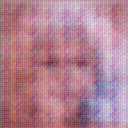
\includegraphics[width=150px]{500_fake_images/samples_5_323.png}%
\caption{A Close Up Of A Black And White Cat}%
\end{figure}

%
\end{document}